%%%%%%%%%%%%%%%%%%%%%%%%%%%%%%%%%%%%%%%%%%%%%%%%%%%%%%%%%%%%%%%%%%%%%%%%%%%%%%%%
\section{Frontera: utilidad dinámica por centro de frontera}%
\label{sec:exp_e1}
%%%%%%%%%%%%%%%%%%%%%%%%%%%%%%%%%%%%%%%%%%%%%%%%%%%%%%%%%%%%%%%%%%%%%%%%%%%%%%%%

La estrategia \textbf{Frontera} calcula el costo dinámico $D(v)$ contando el número de personas detectadas dentro de un radio fijo $r$ alrededor del centroide de la frontera $v$:

\begin{equation}
    D_{\text{Front}}(v) = \bigl|\{ p_i : \| c_v - p_i \|_2 \leq r \}\bigr|
\end{equation}

\noindent La evaluación se realiza en el punto de \emph{destino}, sin considerar el camino que el robot debe recorrer para llegar. Esta simplicidad implica un costo computacional bajo pero también una limitación estructural: el robot puede seleccionar fronteras cuyo entorno inmediato está libre de personas, pero cuyo trayecto de acceso atraviesa zonas concurridas.

\subsection{Diseño de los experimentos}

Los experimentos de validación de la estrategia Frontera comprenden \textbf{10 casos de prueba} (TC001–TC010) con las mismas configuraciones de entorno y densidad de actores que el resto de las etapas de validación, detalladas en la Tabla~\ref{tab:casos_frontera}. Cada caso se ejecutó con \textbf{tres réplicas independientes} (V001–V030); el valor representativo de Frontera en cada configuración es la mediana de las tres réplicas. La línea de base Greedy corresponde a los experimentos G001–G010, ejecutados bajo las mismas condiciones ($\lambda = 5$, $\mu = 0{,}01$, duración 1800 s).

\begin{table}[htbp]
    \centering
    \caption{Casos de prueba de validación: estrategia Frontera y Greedy.}%
    \label{tab:casos_frontera}
    \begin{tabular}{cccrr}
        \toprule
        \textbf{Caso (Frontera)} & \textbf{Caso (Greedy)} & \textbf{Entorno} & \textbf{Actores} & \textbf{Réplicas (Frontera)} \\
        \midrule
        TC001 & G001 & house  &  0 & V001–V003 \\
        TC002 & G002 & office &  0 & V004–V006 \\
        TC003 & G003 & house  &  5 & V007–V009 \\
        TC004 & G004 & office &  5 & V010–V012 \\
        TC005 & G005 & house  & 10 & V013–V015 \\
        TC006 & G006 & office & 10 & V016–V018 \\
        TC007 & G007 & house  & 15 & V019–V021 \\
        TC008 & G008 & office & 15 & V022–V024 \\
        TC009 & G009 & house  & 20 & V025–V027 \\
        TC010 & G010 & office & 20 & V028–V030 \\
        \bottomrule
    \end{tabular}
\end{table}

La normalización global min-máx se aplicó sobre la unión de valores de Frontera y Greedy, con los rangos detallados en la Tabla~\ref{tab:rangos_globales_e1}.

\begin{table}[htbp]
    \centering
    \caption{Rangos globales de normalización para la comparación Frontera vs Greedy.}%
    \label{tab:rangos_globales_e1}
    \begin{tabular}{lrr}
        \toprule
        \textbf{Métrica} & \textbf{Mínimo} & \textbf{Máximo} \\
        \midrule
        Celdas fantasma & 0 & 155 \\
        Entropía del mapa & $9{,}42 \times 10^{-6}$ & $2{,}06 \times 10^{-4}$ \\
        Frames procesados & 98 & 648 \\
        \bottomrule
    \end{tabular}
\end{table}

\noindent El máximo de celdas fantasma (155) corresponde al experimento TC007 (house-15) de la propia estrategia Frontera, lo que constituye un resultado relevante que se discute en la Sección~\ref{sec:exp_e1_discusion}.

\subsection{Resultados por métrica}

La Tabla~\ref{tab:e1_ghost} y la Figura~\ref{fig:e1_ghost} presentan los resultados de celdas fantasma por configuración.

\begin{table}[htbp]
    \centering
    \caption{Celdas fantasma (valor final) por configuración: Frontera vs Greedy. Valores en negrita indican la estrategia ganadora. Menor es mejor.}%
    \label{tab:e1_ghost}
    \begin{tabular}{lrrr}
        \toprule
        \textbf{Configuración} & \textbf{Frontera (mediana)} & \textbf{Greedy} & \textbf{\% dif.} \\
        \midrule
        house-0   & 16              & \textbf{15}  & $+7\%$    \\
        office-0  & 21              & \textbf{13}  & $+62\%$   \\
        house-5   & \textbf{53}     & 81           & $-35\%$   \\
        office-5  & 92              & \textbf{78}  & $+18\%$   \\
        house-10  & \textbf{0}      & 83           & $-100\%$  \\
        office-10 & \textbf{105}    & 125          & $-16\%$   \\
        house-15  & 155             & \textbf{118} & $+31\%$   \\
        office-15 & \textbf{24}     & 153          & $-84\%$   \\
        house-20  & \textbf{0}      & 131          & $-100\%$  \\
        office-20 & \textbf{0}      & 83           & $-100\%$  \\
        \bottomrule
    \end{tabular}
\end{table}

\begin{figure}[htbp]
    \centering
    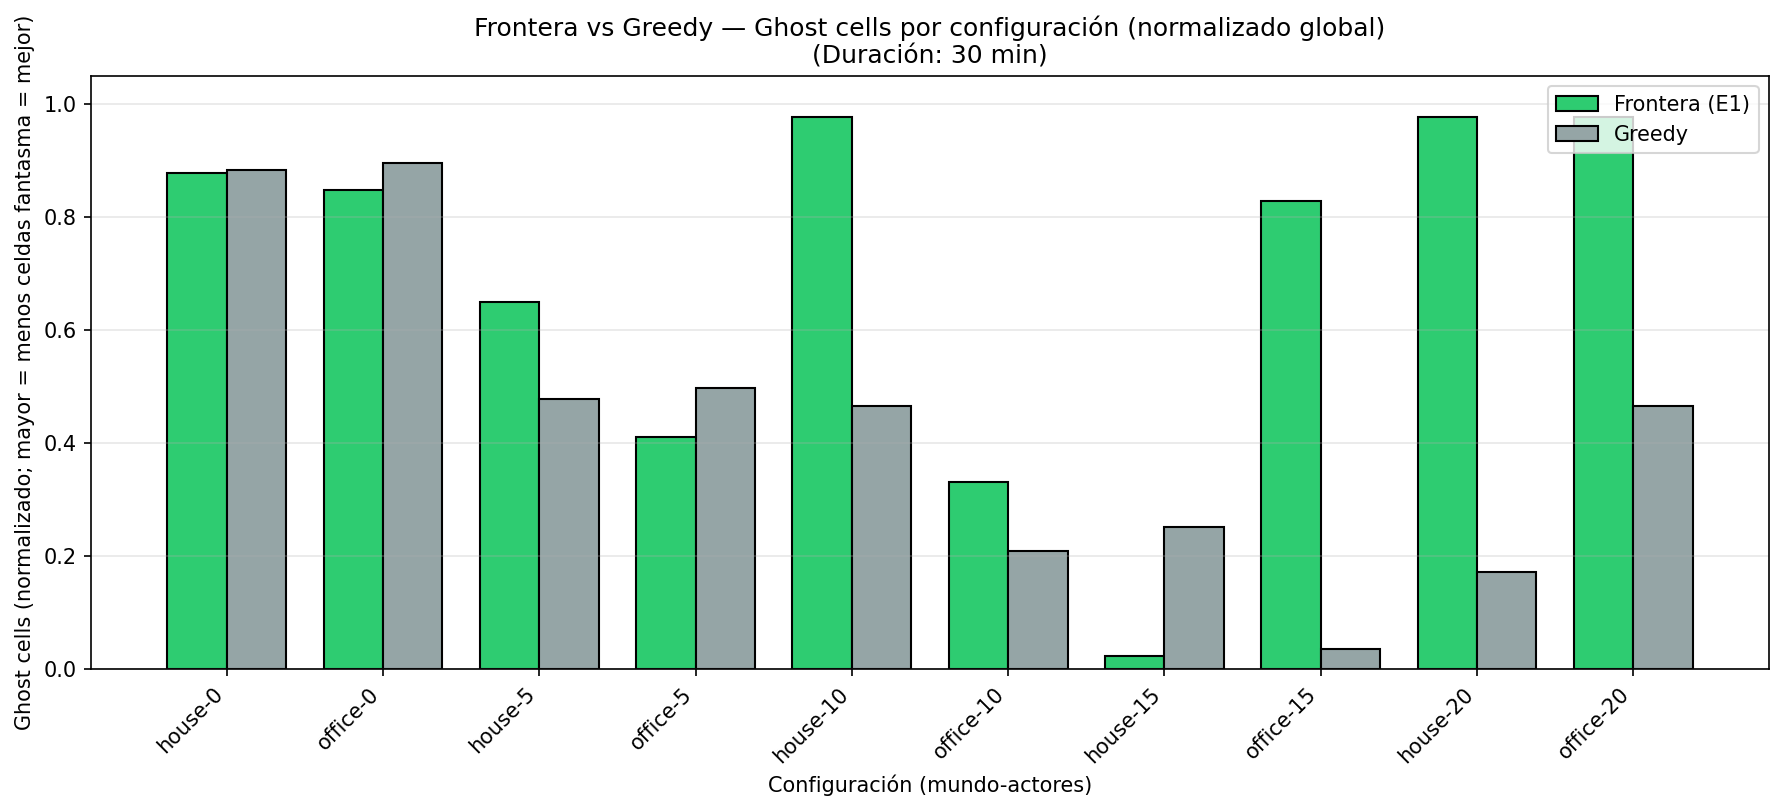
\includegraphics[width=\textwidth]{figures/experiments/frontera/e1_vs_greedy_04_ghost_normalizado.png}
    \caption{Celdas fantasma normalizadas por configuración. Valor normalizado mayor indica menor número de celdas fantasma (mejor precisión del mapa). Frontera supera a Greedy en 6 de las 10 configuraciones.}%
    \label{fig:e1_ghost}
\end{figure}

La estrategia Frontera supera a Greedy en celdas fantasma en \textbf{6 de las 10} configuraciones. Las victorias se concentran en configuraciones con densidad media-alta de actores (10, 15 y 20), donde la estrategia logra cero celdas fantasma en house-10, house-20 y office-20, y reducciones del 84\% en office-15. La excepción más destacada es TC007 (house-15), donde Frontera acumula 155 celdas fantasma frente a 118 de Greedy, el peor resultado individual de toda la estrategia y el máximo global del conjunto de normalización; este caso se analiza en la Sección~\ref{sec:exp_e1_discusion}.

La Tabla~\ref{tab:e1_entropy} y la Figura~\ref{fig:e1_entropy} presentan los resultados de entropía del mapa.

\begin{table}[htbp]
    \centering
    \caption{Entropía del mapa (valor final) por configuración: Frontera vs Greedy. Valores en negrita indican la estrategia ganadora. Mayor es mejor.}%
    \label{tab:e1_entropy}
    \begin{tabular}{lrrr}
        \toprule
        \textbf{Configuración} & \textbf{Frontera (mediana)} & \textbf{Greedy} & \textbf{\% dif.} \\
        \midrule
        house-0   & $\mathbf{1{,}43 \times 10^{-4}}$ & $1{,}29 \times 10^{-4}$ & $+10\%$    \\
        office-0  & $1{,}33 \times 10^{-4}$ & $\mathbf{2{,}06 \times 10^{-4}}$ & $-36\%$   \\
        house-5   & $9{,}5 \times 10^{-5}$  & $\mathbf{1{,}67 \times 10^{-4}}$ & $-43\%$   \\
        office-5  & $7{,}8 \times 10^{-5}$  & $\mathbf{1{,}07 \times 10^{-4}}$ & $-27\%$   \\
        house-10  & $\mathbf{1{,}51 \times 10^{-4}}$ & $6{,}6 \times 10^{-5}$  & $+127\%$  \\
        office-10 & $\mathbf{1{,}49 \times 10^{-4}}$ & $1{,}27 \times 10^{-4}$ & $+17\%$   \\
        house-15  & $\mathbf{1{,}24 \times 10^{-4}}$ & $9{,}4 \times 10^{-6}$  & $+1213\%$ \\
        office-15 & $\mathbf{1{,}12 \times 10^{-4}}$ & $8{,}9 \times 10^{-5}$  & $+26\%$   \\
        house-20  & $4{,}8 \times 10^{-5}$  & $\mathbf{1{,}88 \times 10^{-4}}$ & $-74\%$   \\
        office-20 & $1{,}2 \times 10^{-5}$  & $\mathbf{1{,}21 \times 10^{-4}}$ & $-90\%$   \\
        \bottomrule
    \end{tabular}
\end{table}

\begin{figure}[htbp]
    \centering
    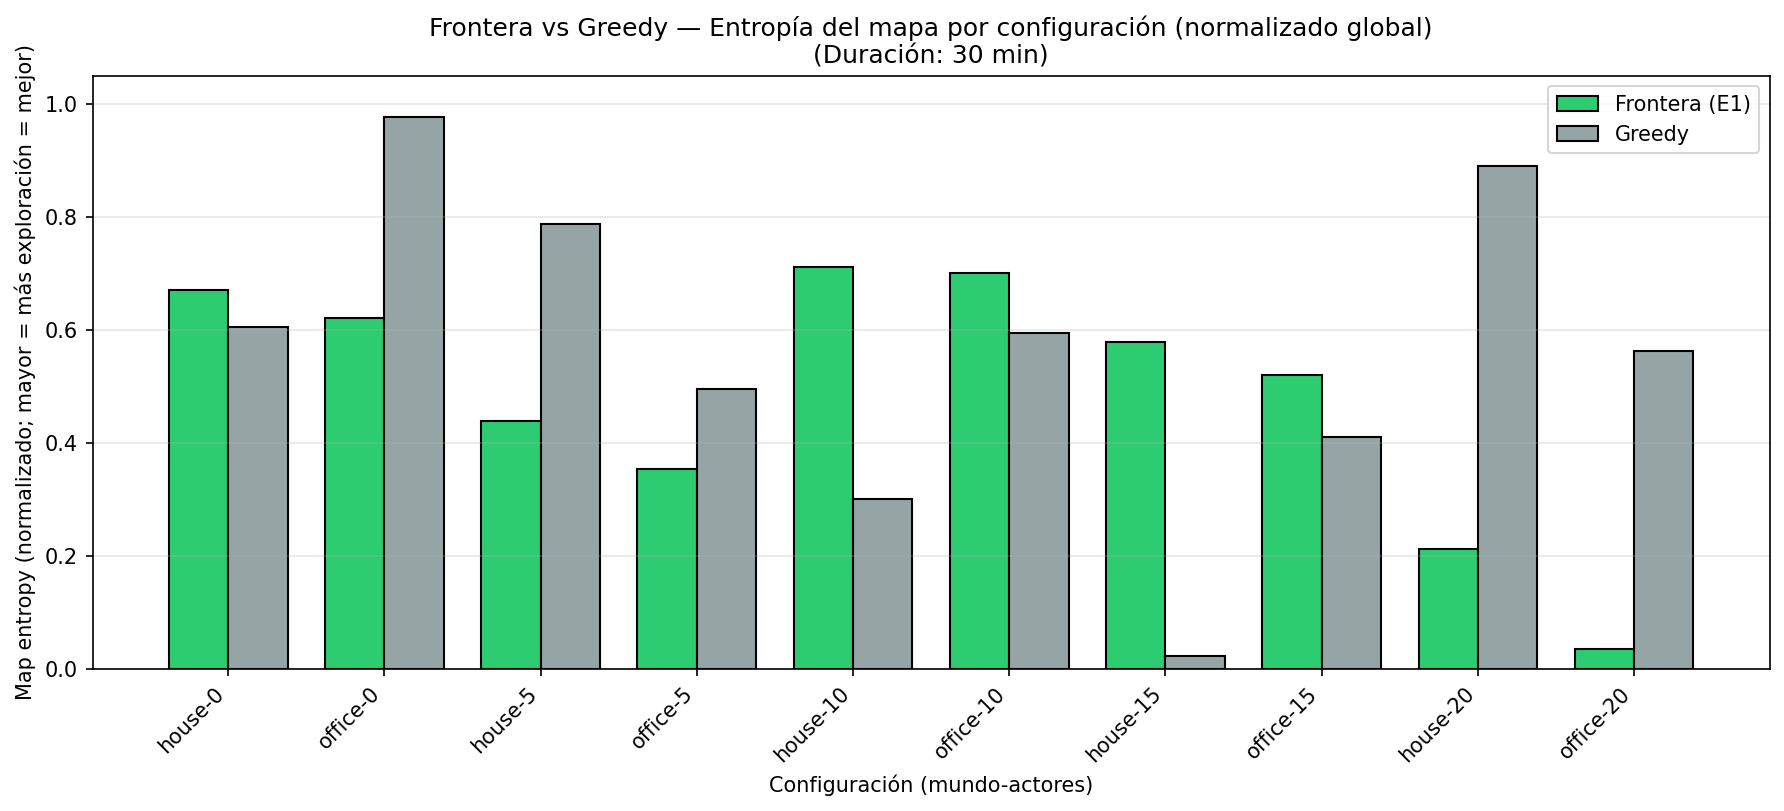
\includegraphics[width=\textwidth]{figures/experiments/frontera/e1_vs_greedy_05_entropy_normalizado.png}
    \caption{Entropía del mapa normalizada por configuración. Valor normalizado mayor indica mayor exploración. Frontera supera a Greedy en 5 de las 10 configuraciones.}%
    \label{fig:e1_entropy}
\end{figure}

En entropía del mapa Frontera supera a Greedy en \textbf{5 de las 10} configuraciones, resultado superior al esperado para una estrategia que solo evalúa el punto de destino. Las victorias se concentran en densidades medias (10 y 15 actores en ambos entornos) y en house-0. En contraste, Greedy domina con claridad en densidad baja (office-0, house-5, office-5) y alta (house-20, office-20), donde la penalización de fronteras por presencia de personas en el destino desorienta la exploración.

La Tabla~\ref{tab:e1_frames} y la Figura~\ref{fig:e1_frames} presentan los resultados de frames procesados.

\begin{table}[htbp]
    \centering
    \caption{Frames totales procesados (valor final acumulado) por configuración: Frontera vs Greedy. Valores en negrita indican la estrategia ganadora. Mayor es mejor.}%
    \label{tab:e1_frames}
    \begin{tabular}{lrrr}
        \toprule
        \textbf{Configuración} & \textbf{Frontera (mediana)} & \textbf{Greedy} & \textbf{\% dif.} \\
        \midrule
        house-0   & \textbf{364}  & 217  & $+68\%$   \\
        office-0  & 478           & \textbf{555} & $-14\%$  \\
        house-5   & 439           & \textbf{577} & $-24\%$  \\
        office-5  & 444           & \textbf{648} & $-31\%$  \\
        house-10  & 390           & \textbf{454} & $-14\%$  \\
        office-10 & 400           & \textbf{601} & $-33\%$  \\
        house-15  & 356           & \textbf{597} & $-40\%$  \\
        office-15 & 366           & \textbf{607} & $-40\%$  \\
        house-20  & \textbf{353}  & 265  & $+33\%$   \\
        office-20 & \textbf{379}  & 98   & $+287\%$  \\
        \bottomrule
    \end{tabular}
\end{table}

\begin{figure}[htbp]
    \centering
    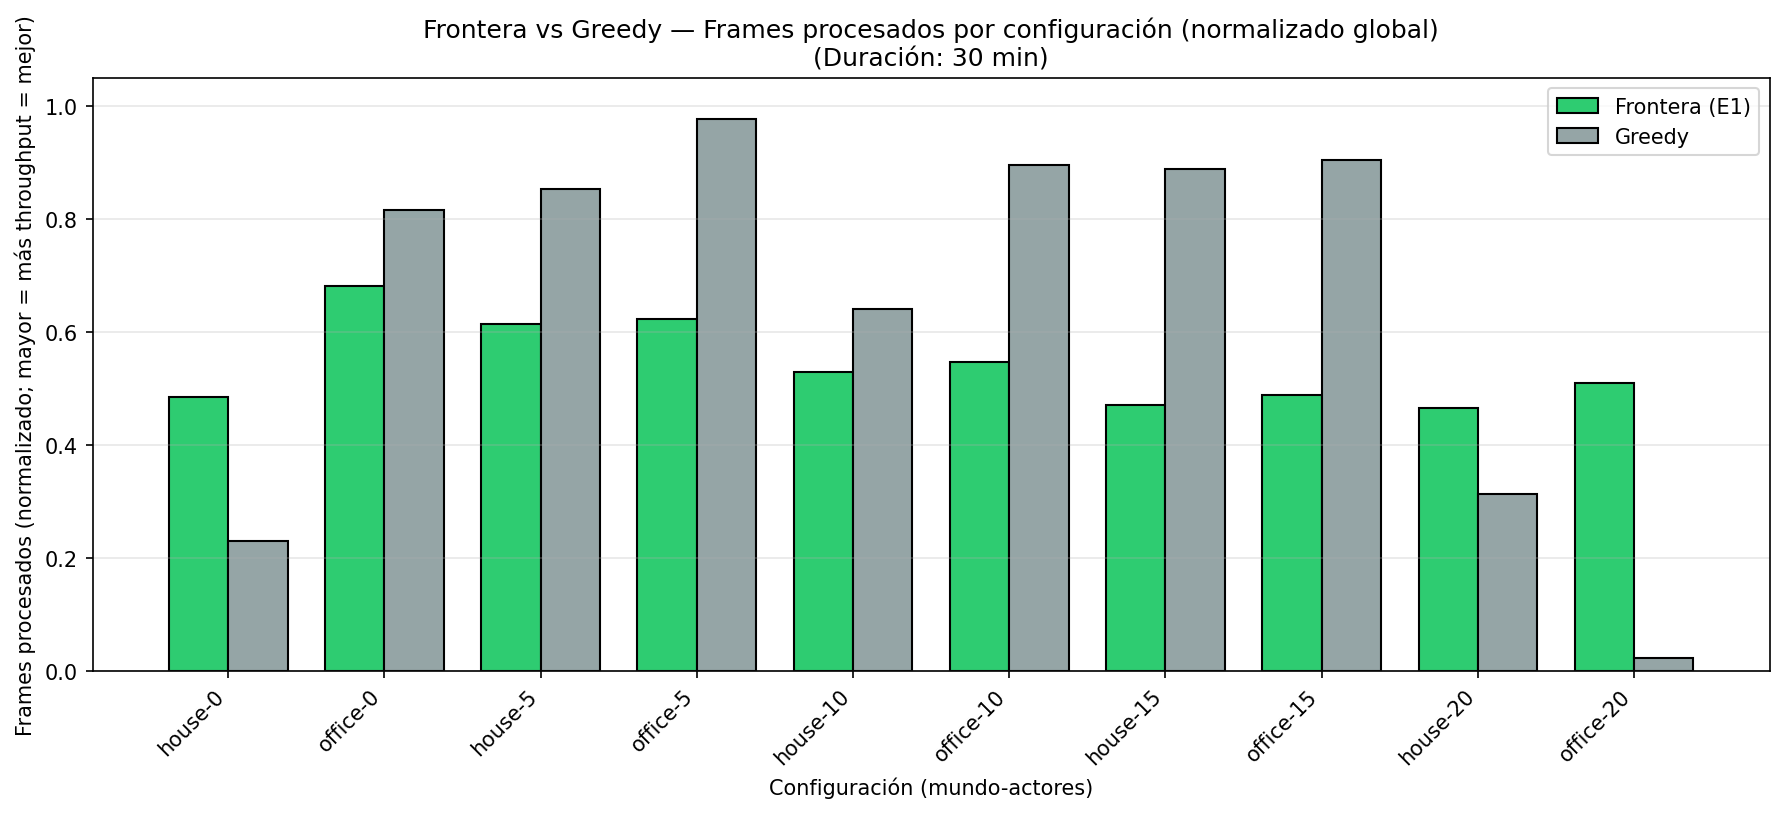
\includegraphics[width=\textwidth]{figures/experiments/frontera/e1_vs_greedy_06_frames_normalizado.png}
    \caption{Frames procesados normalizados por configuración. Valor normalizado mayor indica mayor throughput del pipeline de visión. Frontera supera a Greedy en 3 de las 10 configuraciones.}%
    \label{fig:e1_frames}
\end{figure}

En frames procesados Frontera supera a Greedy únicamente en \textbf{3 de las 10} configuraciones: house-0 ($+68\%$), house-20 ($+33\%$) y office-20 ($+287\%$). En las siete configuraciones restantes —todas de densidad baja a media— Greedy procesa significativamente más frames, con diferencias del $-14\%$ al $-40\%$. El patrón de victoria en los extremos de densidad (0 y 20 actores) se discute en la Sección~\ref{sec:exp_e1_discusion}.

\subsection{Puntuación compuesta y análisis global}

Las Figuras~\ref{fig:e1_score_config} y~\ref{fig:e1_victorias} resumen los resultados por puntuación compuesta.

\begin{figure}[htbp]
    \centering
    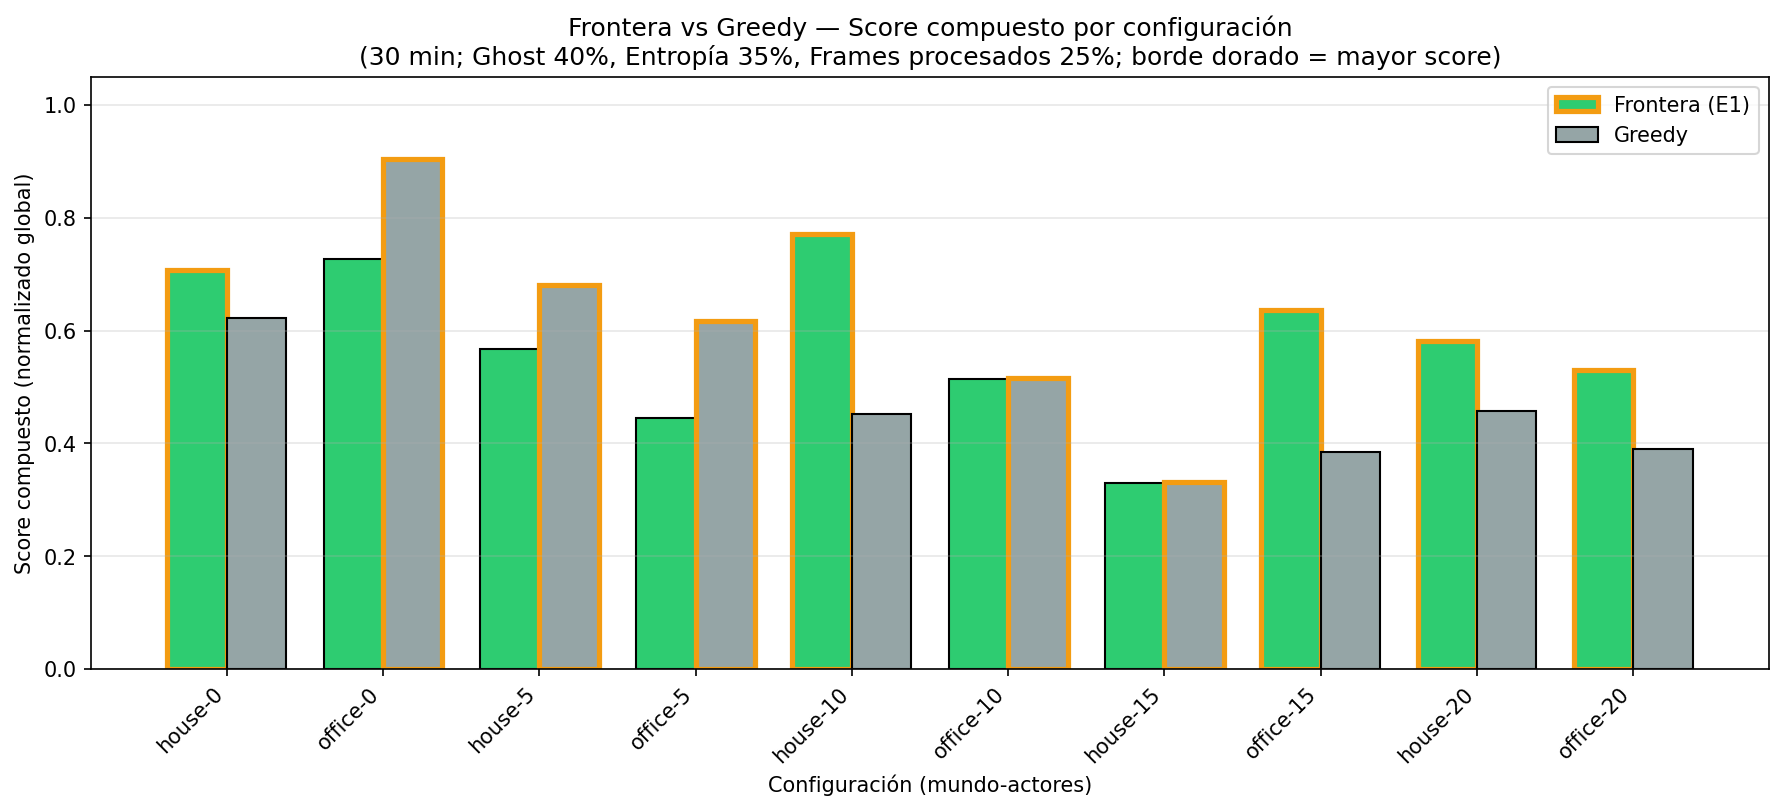
\includegraphics[width=\textwidth]{figures/experiments/frontera/e1_vs_greedy_01_score_por_config.png}
    \caption{Puntuación compuesta por configuración (Frontera vs Greedy). Pesos: celdas fantasma 40\%, entropía 35\%, frames 25\%. Frontera supera a Greedy en 5 de las 10 configuraciones.}%
    \label{fig:e1_score_config}
\end{figure}

\begin{figure}[htbp]
    \centering
    \begin{subfigure}[b]{0.60\textwidth}
        \centering
        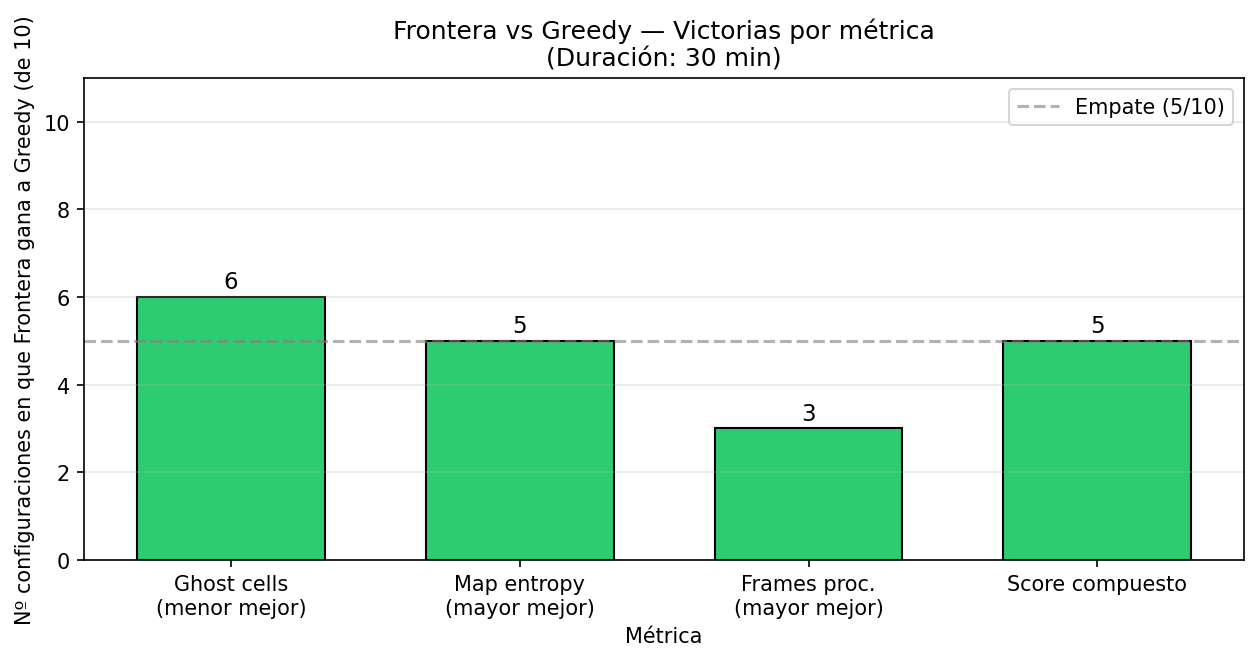
\includegraphics[width=\textwidth]{figures/experiments/frontera/e1_vs_greedy_02_victorias_por_metrica.png}
        \caption{Victorias por métrica individual.}
    \end{subfigure}
    \hfill
    \begin{subfigure}[b]{0.36\textwidth}
        \centering
        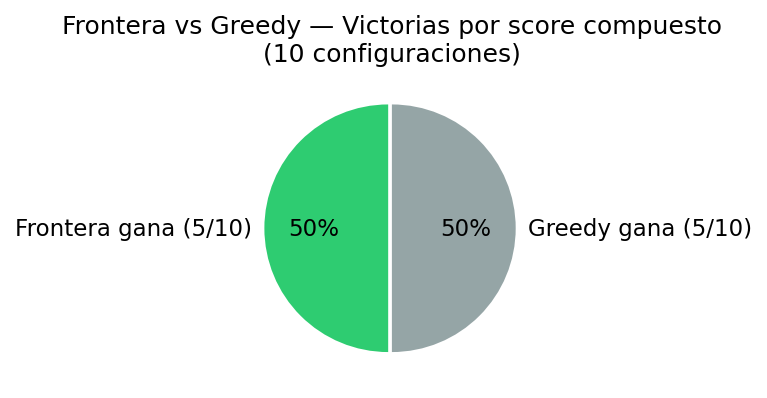
\includegraphics[width=\textwidth]{figures/experiments/frontera/e1_vs_greedy_03_torta_victorias_score.png}
        \caption{Victorias por puntuación compuesta.}
    \end{subfigure}
    \caption{Resumen de victorias de la estrategia Frontera frente a Greedy.}%
    \label{fig:e1_victorias}
\end{figure}

Por puntuación compuesta, la estrategia Frontera es ganadora en \textbf{5 de las 10} configuraciones: TC001 (house-0), TC005 (house-10), TC008 (office-15), TC009 (house-20) y TC010 (office-20). En las cinco configuraciones restantes Greedy obtiene mayor puntuación; cuatro de ellas corresponden a office-0, house-5, office-5 y office-10, y la quinta a house-15, donde Frontera registra su peor resultado en ghost cells.

Aplicando el criterio de cuasi-empate ($S_{\text{Front}} \geq 0{,}9 \cdot S_{\text{Greedy}}$), Frontera resulta competitiva o mejor en \textbf{7 de las 10} configuraciones, lo que indica que incluso en los casos en que Greedy supera a Frontera, la diferencia en puntuación compuesta es reducida en la mayoría de ellos.

\subsection{Análisis por entorno}

\textbf{Entorno house.} En celdas fantasma, Frontera supera a Greedy en house-5, house-10 y house-20, pierde en house-0 por un margen mínimo (16 vs 15) y registra su peor caso en house-15 (155 vs 118). En entropía, Frontera gana en house-0, house-10 y house-15, y pierde en house-5 y house-20. En frames, solo supera a Greedy en house-0 y house-20. La puntuación compuesta favorece a Frontera en TC001, TC005 y TC009 (house-0, house-10 y house-20).

\textbf{Entorno office.} En celdas fantasma, Frontera supera a Greedy en office-10, office-15 y office-20, y pierde en office-0 y office-5. En entropía, gana en office-10 y office-15, y pierde en office-0, office-5 y office-20. En frames, solo supera a Greedy en office-20 ($+287\%$). La puntuación compuesta favorece a Frontera en TC008 y TC010 (office-15 y office-20).

En conjunto, el beneficio de la estrategia Frontera aumenta con la densidad de actores en ambos entornos, con la excepción de house-15 que constituye un caso anómalo. Las configuraciones con 20 actores muestran las ventajas más consistentes tanto en ghost cells como en frames procesados.

\subsection{Discusión}%
\label{sec:exp_e1_discusion}

Los resultados permiten identificar tres aspectos centrales del comportamiento de la estrategia Frontera:

\textbf{Precisión del mapa.} La evaluación de personas en el entorno inmediato del centro de la frontera es efectiva para reducir ghost cells en la mayoría de las configuraciones con actores, especialmente a densidades de 10 o más. Sin embargo, la estrategia ignora el trayecto de acceso: el robot puede seleccionar una frontera libre de personas pero atravesar zonas concurridas durante el camino, generando ghost cells en el recorrido. Este mecanismo explica tanto las victorias parciales como las pérdidas en configuraciones de densidad media donde las personas se concentran en los pasillos de acceso más que en las propias fronteras.

\textbf{La anomalía de house-15.} El caso TC007 (house-15) presenta el peor resultado de toda la estrategia: 155 celdas fantasma frente a 118 de Greedy. Con 15 actores en el entorno compacto de house, la alta densidad de personas cerca de múltiples fronteras candidatas puede provocar que la estrategia descarte sistemáticamente las fronteras más accesibles en favor de alternativas más lejanas que, al momento de llegar, ya se encuentran igualmente ocupadas. Este efecto de degradación por sobrepenalización es propio de estrategias que evalúan solo el punto de destino sin anticipar el estado futuro.

\textbf{Frames procesados y densidad extrema.} El patrón de victorias en frames a 0 y 20 actores responde a mecanismos distintos. Con 0 actores, la ausencia de personas elimina cualquier penalización dinámica y Frontera puede orientar su exploración hacia fronteras que maximizan el tiempo de observación activa. Con 20 actores, evitar las zonas más congestionadas permite al robot mantener un desplazamiento más fluido con menos interrupciones, procesando más frames en el mismo tiempo. En densidades intermedias (5–15 actores), la penalización de fronteras reduce la eficiencia de movimiento sin ofrecer un beneficio proporcional en frames.

En conjunto, los resultados validan la estrategia Frontera como alternativa competitiva a Greedy cuando se prioriza la precisión del mapa a densidades medias y altas, con la salvedad de que su comportamiento es menos predecible en configuraciones específicas donde la distribución espacial de los actores interactúa negativamente con el mecanismo de evaluación por centro de frontera.
